\chapter{Introduction}
Urban development drastically changes the character of the surface. Replacement of natural terrain with roads, buildings, parks, and other urban features modifies the geometry of the surface as well as its thermal, radiative, moisture, and aerodynamic properties. These modifications, combined with anthropogenic emissions of heat, result in a distinct urban climate; one which is often warmer, a phenomenon termed the urban heat island effect (UHI). As both the Earth's population and the urbanized fraction of that population increase \citep{Nations2014}, cities grow and more people are exposed to urban-modified atmospheres. Thus, understanding how cities interact with the climate across spatiotemporal scales has important implications for human health, energy efficiency, and for informing future urban development. This, in part, has prompted significant expansion in study of the urban effect on climates, particularly in the decades preceding this thesis. 

The notion that urban areas have elevated air and surface temperatures (T\textsubscript{air} and T\textsubscript{surf} respectively) is not new, with the first formal studies of the urban effect on T\textsubscript{air} dating back to \citet{Howard1833}'s identification of "artificial warming" and "urban contamination" in his characterization of spatial patterns of T\textsubscript{air} in early 19\textsuperscript{th} century London. Conceptually, contemporary studies of urban climate do not stray far from \citet{Howard1833}, by seeking to isolate and quantify the urban signal in measured or modeled assessment of a given meteorological variable. However, as \citet{Howard1833} identified nearly two centuries ago, the sheer number of factors influencing direct measurement of climates makes experimental control nearly impossible in observational study. In any given observation of climate, myriad urban and non urban signals make it difficult to determine what is urban and what is not, degrading interstudy comparison. Even in the modeling domain, where experimental control is possible, the inherent complexity in simulating flows of energy, momentum, and mass at the scales necessary to represent physical phenomena over realistic urban environments is, as of yet, not possible. Notwithstanding implementation of accurate, physically based schemes to represent urban climates in regional or global climate models. Thus, accurate assessment how a city affects the climate is a deceptively challenging task. To address this, \citet{Lowry1977} presents a framework to isolate the urban effect in observation of a given meteorological variable. In his framework - termed the "Lowry method" - measurement of a meteorological variable ($V_M$) is the sum of forcings from the background climate and synoptic conditions ($V_B$), local topography ($V_L$), and the urban landscape ($V_H$)

\begin{equation}
	V_M = V_B + V_L + V_H
\end{equation}

Thus, isolation of the urban effect on observed $V_M$ simply requires the removal of $V_B$ and $V_L$. This can be achieved by subtracting some urban affected observation ($V_{M, U}$) from a non-urban observation ($V_{M, R}$) where $V_{H, R}$ = 0,

\begin{equation}
V_{M, U} - V_{M, R} = (V_B + V_L + V_H) - (V_B + V_L) = V_H
\end{equation}

\noindent simplified as,

\begin{equation}
	V_H = V_{M, U} - V_{M, R}
\end{equation}

Study of the urban heat island effect tacitly falls into such a framework, by replacing $V_{M, U} - V_{M, R}$ with $\Delta$T\textsubscript{air, U-R}. However, in spite of its conceptual simplicity through the lens of the Lowry method, meta-analysis of observational air temperature UHI (aUHI) study suggests that that simplicty may not translate well to real world analysis. In his analysis of the aUHI literature, \citet{Stewart2011} found that nearly fifty percent of aUHI studies published between 1950 and 2007 are "scientifically indefensible" based on an analysis of relevant criteria\footnote{Each study was given a "passing" or "failing" grade and ranked using a points-based scheme to assess methodological quality in the following criteria: conceptual model, operational definitions, instrument specification, site metadata, site representativeness, number of replicates, weather control, surface control, and synchronicity.}, suggesting a significant gulf between conceptual simplicity and practical realities in aUHI analysis. Of the 190 surveyed studies, only 13\% were derived from field sites that were sufficiently representative of the local-scale environment or lacked the meta-data to make such a determination, leading to potential biases from micro-scale terrain. This is particularly discouraging as it is not the result of an evolution in measurement techniques or improved instrumentation, as techniques to observe and analyze aUHI did not see significant evolution since 1950 - in fact, \citet{Stewart2011} suggests the opposite: a disproportionately large number of studies deemed scientifically sound were published early in the study purview. Thus, in study of the urban effect on variables for which significant methodological shifts have or will occur, the warnings implicit in \citet{Stewart2011} are particularly salient, as inherent difficulties found in translating "Lowry"-esque conceptual models to real world observations may be compounded by significant methodological changes. In the five years since its publication, aUHI study has seen further expansion and, as such, it is difficult to assess whether its critical analysis has prompted a shift towards more thoughtful, careful, and methodical study of aUHI, notwithstanding its relevance in study of the urban effect on different meteorological variables.

In contrast to study of urban T\textsubscript{air}, the introduction of new methods, instruments, and analytical techniques in TIR remote sensing of urban environments has lead to rapid evolution in study of the urban effect on land T\textsubscript{surf} - a vast majority of which has focused on passive remote sensing of upwelling TIR. In the decades preceding this thesis, a combination of factors has lead to an increased focus on remote sensed study of urban T\textsubscript{surf}: 

\begin{itemize}
	\item The proliferation of satellite and aerial thermal infrared (TIR) remote sensors and "openness" in data access policies.
	\item Improvements in sensor spatial, spatial, and radiometric resolutions. 
	\item An increased focus on the importance of the surface in both determining and understanding key near-ground micro-meteorological phenomena.
\end{itemize}

Remote sensed study of the urban effect on land T\textsubscript{surf} has been instrumental in characterizing large-scale spatial and temporal patterns of sUHI \citep{Peng2012, Streutker2003, Imhoff2010}. However, the methodological and conceptual concerns raised in \citet{Stewart2011} in combination with the wide (and broadening) range of methodologies for remote sensed urban T\textsubscript{surf} retrieval should prompt critical assessment of the remote sensed sUHI literature. Difficulties suggested in \citet{Stewart2011} may be amplified by methodological shifts and a variety of methods for analysis. At the time of writing, no systemic or critical reviews of the remote sensed sUHI literature are available. An increasingly dogmatic focus on improving spatial and radiometric resolutions has left other inherent biases in remote sensing of urban environments largely ignored in sUHI literature. This suggests that similar conclusions to those found of aUHI literature in \citet{Stewart2011} are possible (if not likely) for study of sUHI. 

Traditional methods for urban T\textsubscript{surf} measurement are subject to a suite of geometric and temporal biases. These biases are largely inherent to the discipline and contribute an additional source of error on top of potential concerns carried over from meta-analysis of conceptual flaws in aUHI literature. 

Geometric biases in TIR remote sensing of the urban surface are the result of urban modification of surface structure and thermal and radiative properties. Relative to typical non-urban and rural terrain, urban development adds significant 3-dimensionality to the surface. This added complexity results in undersampling of the surface by narrow-FOV remote sensors. A narrow-FOV sensor, by sampling surface 3-dimensionality in 2-dimensions, "sees" a different assemblage of urban surfaces depending on its viewing direction, resulting in a geometric bias towards some arrangement of facets. I.e. viewing from the nadir, a narrow-FOV sensor sees the urban surface as an array of rooftops and roads, the same sensor viewing perpendicular to the surface sees wall facets exclusively, and one viewing from some off nadir angle sees some array of walls, rooftops, and roads depending on its orientation. 

In addition, the convoluted 3-dimensional structure of the urban surface modifies sunlit/shading regimes, resulting in strong micro-scale spatiotemporal contrasts in urban T\textsubscript{surf}, which depend on surface-sun geometry. These microscale variations in urban T\textsubscript{surf} are often amplified by significant directional contrasts in the thermal admittance of common urban materials, which determines the diurnal amplitude of T\textsubscript{surf} for a given facet. Thus, when viewed from a narrow-FOV remote sensor with some inherent geometric bias, urban T\textsubscript{surf} is directionally dependent - constituting an "effective anisotropy" of urban T\textsubscript{surf}, shown in Figure \ref{anisot}. The qualifier "effective" is used to differentiate directional contrasts in urban T\textsubscript{surf} that arise from a city's 3-dimensional surface structure from those resulting from the non-Lambertian nature of individual urban facets (e.g. walls, rooftops, or roads). The magnitude of urban effective anisotropy can reach up to 10 \si{\kelvin} and is highly dependent on surface-sensor-sun geometry, surface structure, and urban materials \citep{Krayenhoff2016, Voogt1997}. 

\begin{figure}[H]
	\centering
	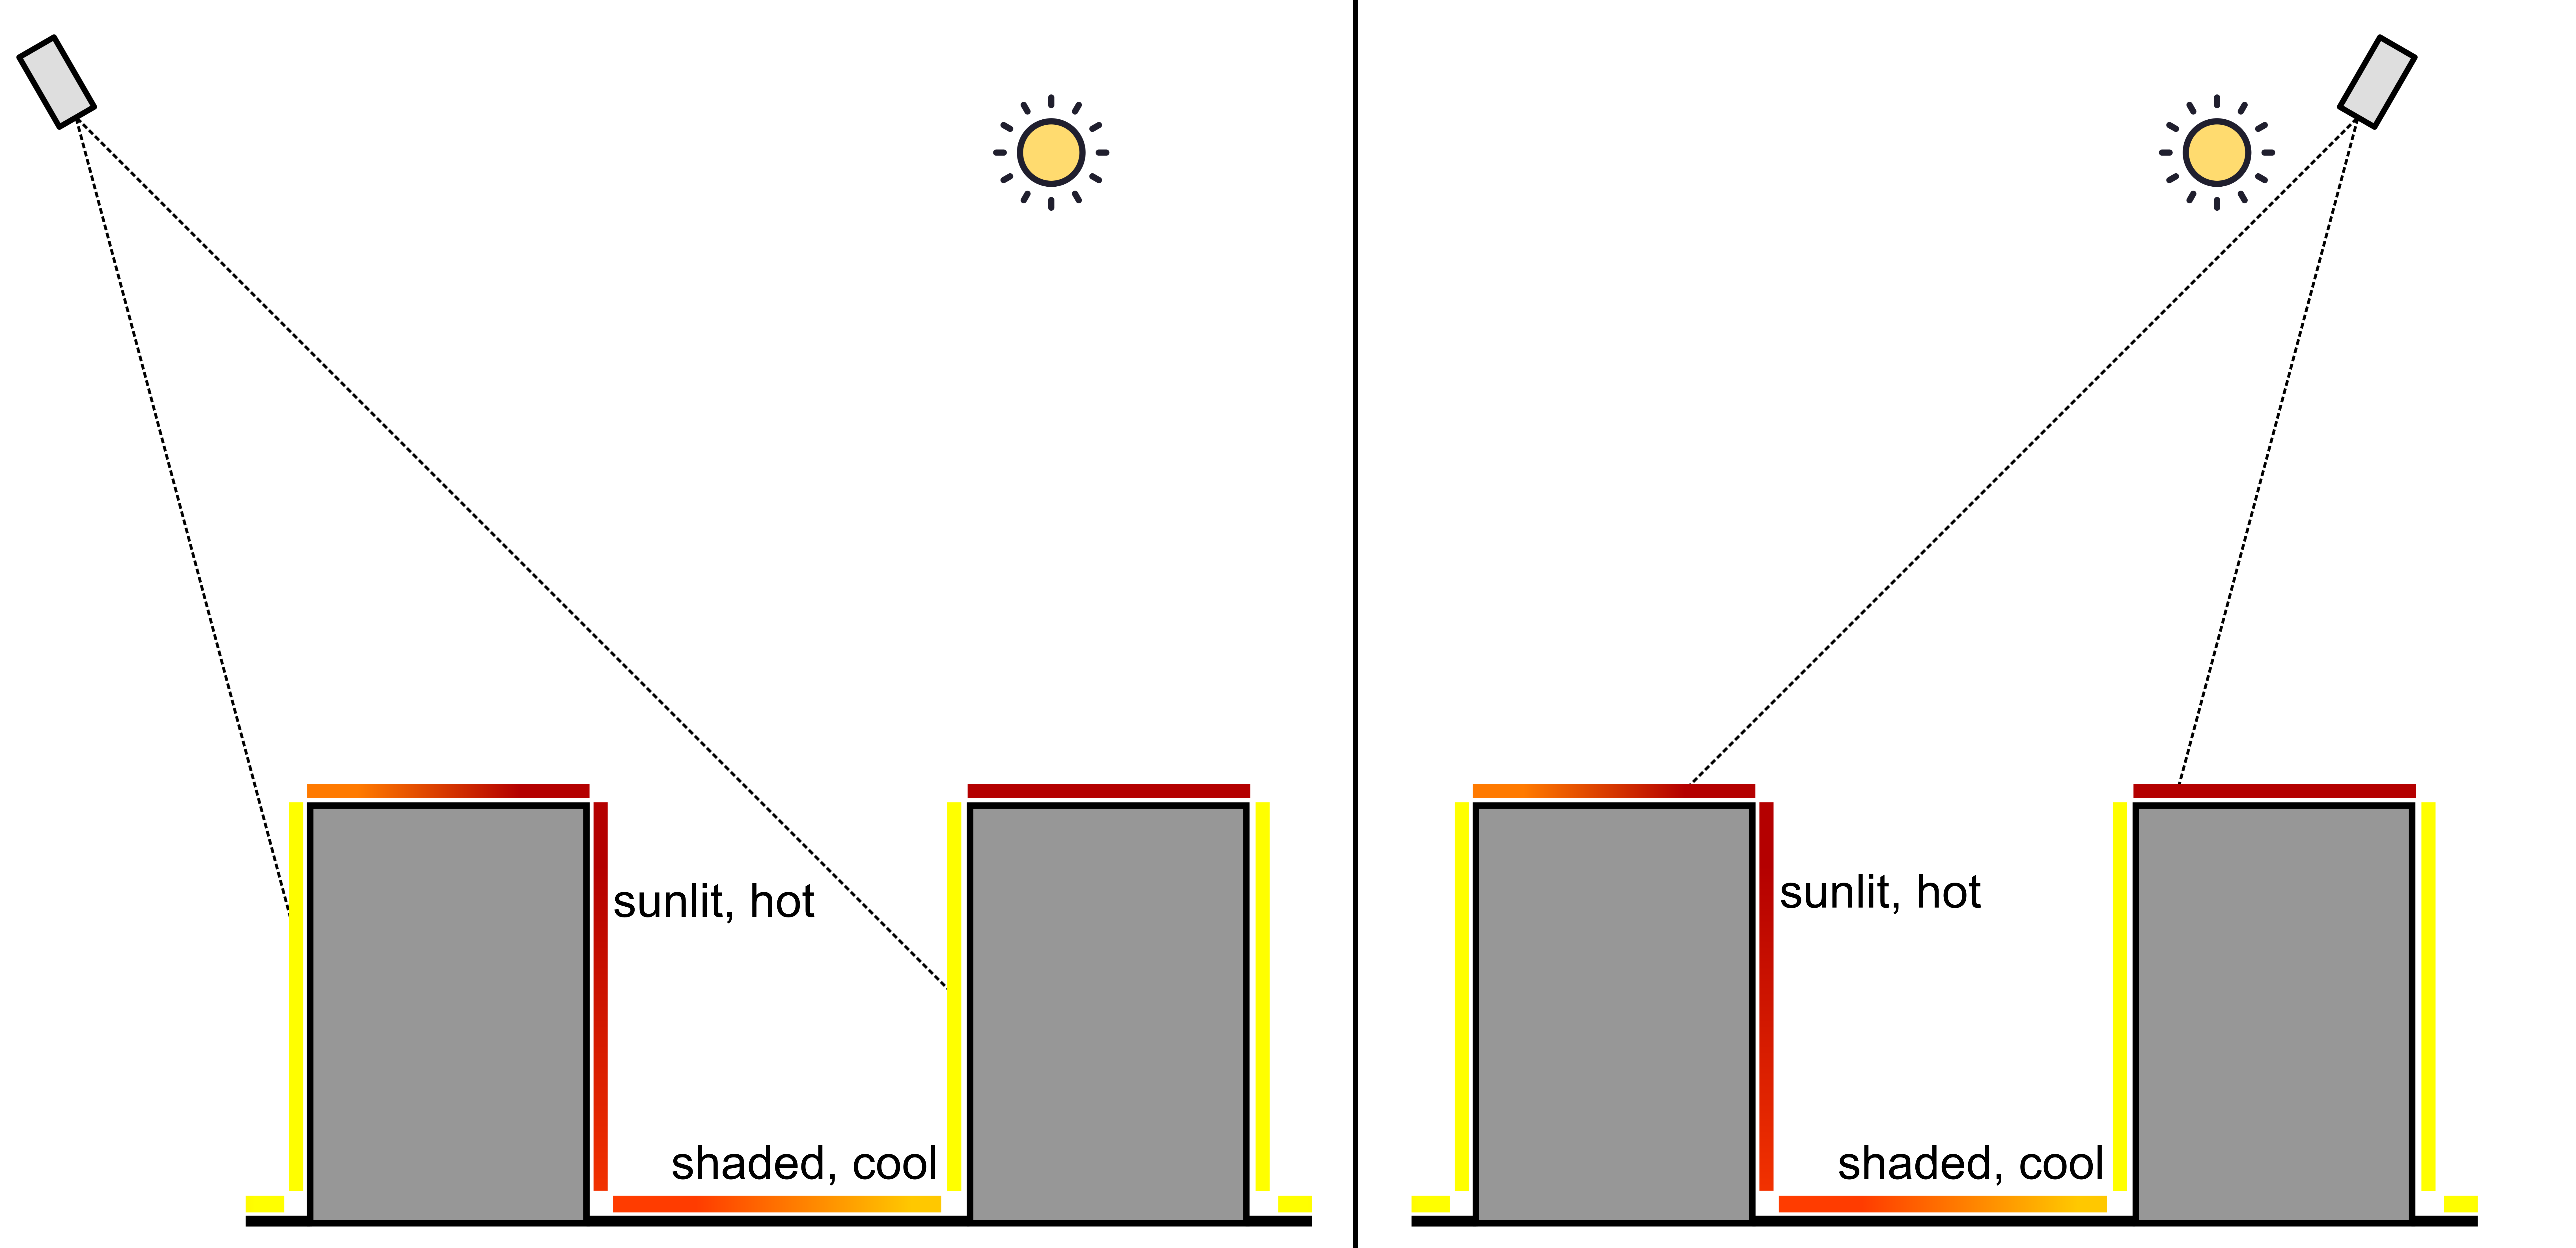
\includegraphics[width=15cm,
	height=7in,
	keepaspectratio]{anisot}
	\caption{A narrow-FOV sensor viewing an idealized urban surface from two angles. Left: viewing the surface approximately perpendicular to the sun's angle. Right: viewing the surface approximately parallel to the sun's angle. The two viewing angles described in the left and right panels yield different remote sensed T\textsubscript{surf} by sampling different arrangements of sunlit and shaded features. Both will deviate from an area weighted "complete" urban T\textsubscript{surf}.}
	\label{anisot}
\end{figure}

Geometric undersampling by narrow-FOV remote sensors results in remote sensed urban T\textsubscript{surf} changing based on a sensor's viewing direction and the assemblage facets included within the sensor FOV. A sensor viewing the surface perpendicular (parallel) to the sun's angle will tend to underestimate (overestimate) the "true" complete urban surface temperature - often calculated as an area weighted average of wall, rooftop, and road T\textsubscript{surf} - by differentially biasing sunlit or shaded facets. Similarly, a sensor in the nadir will tend to overestimate daytime urban T\textsubscript{surf} and underestimate nighttime T\textsubscript{surf}, from a bias towards differentially hot (cool) rooftop facets by day (night) and a neglect of wall facets which are differentially cooler (warmer) by day (night). As the effect of geometric biases is highly dependent on surface-sensor-sun geometry and requires significant instrumentation for quantification, its influence in the remote sensed sUHI record is presently unknown.

Temporal biases in thermal remote sensing of urban areas occur across multiple time scales including: 

\noindent---\textit{Contamination by turbulence forced, high frequency fluctuations in urban T\textsubscript{surf}}. 

Using time-sequential thermography \citet{Christen2012} found that many common urban fabric types (e.g. rooftops, walls, roads, and vegetation) display large micro-scale (second to minute) fluctuations in T\textsubscript{surf}. The magnitude of which is inversely related to surface thermal admittance and is, as of writing, poorly understood. Most thermal remote sensors provide instantaneous, rather than temporally averaged, T\textsubscript{surf} and thus are subject to contamination by high-frequency fluctuations. These biases are difficult to estimate in urban environments, where a large variety of fabric materials can produce significant directional contrasts in thermal admittance - and thus spatial variations in the magnitude of microscale fluctuations depending on the facet material types viewed by the sensor. 

\noindent---\textit{Discontinuity in satellite overpass cycles.}

Satellite overpass cycles are discontinuous. Assessment of land T\textsubscript{surf} either sacrifices spatial resolution for a daily repeat cycle - as is the case with MODIS  - or sacrifices temporal resolution for a higher spatial resolution - ASTER or Landsat. Geostationary satellites do not currently have sufficient spatial resolution to resolve coherent urban pixels.

\noindent---\textit{Clear-sky bias.}

Clouds absorb TIR – thus satellite TIR remote sensing of the surface requires clear sky conditions. Although the urban effect on T\textsubscript{surf} is most evident under "satellite friendly" clear sky conditions (manifesting as large sUHI magnitudes), a clear sky bias likely entails overestimation of "all-sky" sUHI and further adds to discontinuities in the remote sensed urban T\textsubscript{surf} record.

As is the case with geometric biases, the magnitude of these temporal biases in remote sensed urban T\textsubscript{surf} is difficult to quantify without long-term ground truthing campaigns or significant interpolation. Thus, the true temporal and geometric nature of urban effect of T\textsubscript{surf} is presently unknown.
 
\section{Research questions and objectives}

Prompted by these shortcomings in the remote sensed urban T\textsubscript{surf} record, this thesis introduces a method to provide geometrically representative, temporally continuous urban T\textsubscript{surf} for sUHI analysis to address the following questions:

\begin{itemize}
	\item What is the nature of urban surface temperature when viewed from a hemispherical downward-facing radiometer? And how does it relate to urban temperatures derived from other methods for urban surface temperature retrieval?
	\item What is the diurnal and seasonal nature of the surface urban heat island effect?
\end{itemize}

\noindent In an attempt to answer these questions, I did the following:

\begin{enumerate}
	\item Developed and evaluated a method to retrieve atmospherically correction hemispherical radiometric urban surface temperatures from time-continuous measurements of upwelling longwave radiation.
	\item Compared urban surface temperatures and surface urban heat island magnitudes retrieved using the method to common remote sensed representations of the urban surface.
	\item Derived an eight month climatology of hemispherical urban surface temperatures to observe seasonal and diurnal patterns of the surface urban heat island effect.
\end{enumerate}

\section{The structure of the following sections}

The following two papers make up the body of the thesis, read them you fuck.